\ylDisplay{Mootorratas} % Ülesande nimi
{Tundmatu autor} % Autor
{lahtine} % Voor
{2007} % Aasta
{G 5} % Ülesande nr.
{2} % Raskustase
{
% Teema: Dünaamika
\ifStatement
Mootorrattur tahab hüpata üle kraavi, mille mõõtmed on näidatud joonisel. Kui suur peab olema mootorratturi minimaalne kiirus $v$ lennu alguses selleks, et tema ettevõtmine õnnestuks?

\begin{center}
	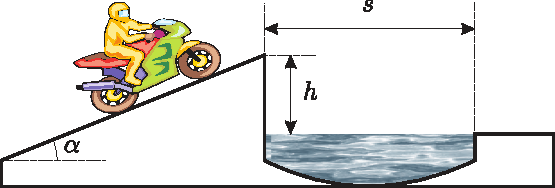
\includegraphics[width=0.8\linewidth]{2007-lahg-05-yl}
\end{center}
\fi


\ifHint
Tegu on suhteliselt sirgjoonelise ballistilise probleemiga. Mootorratturi kiirus peab olema selline, et mootorratturi paraboolne trajektoor läbiks kraavi vastasnurka.
\fi


\ifSolution
Suuname koordinaatteljed nii, nagu näidatud joonisel.

\begin{center}
	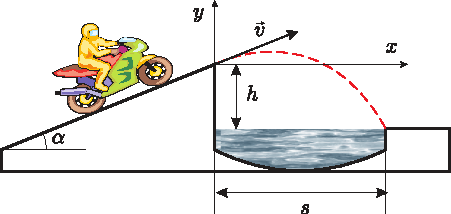
\includegraphics[width=0.8\linewidth]{2007-lahg-05-lah}
\end{center}

Mootorratturi liikumist kirjeldavad seosed
\[
x=v t \cos \alpha, \quad y=v t \sin \alpha-\frac{g t^{2}}{2},
\]
kust saame
\[
y=x \tan \alpha-\frac{g x^{2}}{2 v^{2} \cos ^{2} \alpha}.
\]
See on parabooli võrrand. Asendades siia mootorratturi langemiskoha koordinaadid $x = s$ ja $y = -h$, leiame minimaalse kiiruse
\[
-h=s \tan \alpha-\frac{g s^{2}}{2 v^{2} \cos ^{2} \alpha} \Rightarrow \frac{g s^{2}}{2 v^{2} \cos ^{2} \alpha}=h+s \tan \alpha \Rightarrow
\]
\[
\Rightarrow \quad 2 v^{2} \cos ^{2} \alpha=\frac{g s^{2}}{h+s \tan \alpha} \quad \Rightarrow \quad v^{2}=\frac{g s^{2}}{2 \cos ^{2} \alpha(h+s \tan \alpha)} \quad \Rightarrow
\]
\[
v=\frac{s}{\cos \alpha} \sqrt{\frac{g}{2(h+s \tan \alpha)}}.
\]
\fi
}